\documentclass[10pt]{article}
\usepackage[ngerman]{babel}
\usepackage[utf8]{inputenc}
\usepackage[T1]{fontenc}
\usepackage{graphicx}
\usepackage[export]{adjustbox}
\graphicspath{ {./images/} }
\usepackage{amsmath}
\usepackage{amsfonts}
\usepackage{amssymb}
\usepackage[version=4]{mhchem}
\usepackage{stmaryrd}

\title{Hauptprüfung Abiturprüfung 2022 - Leistungsfach }

\author{Alexander Schwarz\\
www.mathe-aufgaben.com}
\date{}


\begin{document}
\maketitle
 Baden-WürttembergJuni 2022

\section*{Aufgabe C2}
Beim einmaligen Drehen des abgebildeten Glücksrads erhält man eine von vier möglichen Punktzahlen. Die Tabelle gibt für jede Punktzahl die zugehörige Wahrscheinlichkeit an.\\
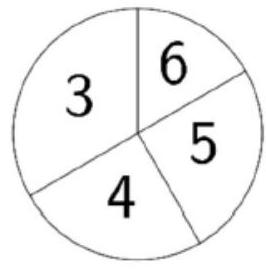
\includegraphics[max width=\textwidth, center]{2025_04_24_3ee02515fbfa521019f2g-2}

\begin{center}
\begin{tabular}{|l|c|c|c|c|}
\hline
Punktzahl & 3 & 4 & 5 & 6 \\
\hline
Wahrscheinlichkeit & $\frac{1}{3}$ & $\frac{1}{4}$ & $\frac{1}{4}$ & $\frac{1}{6}$ \\
\hline
\end{tabular}
\end{center}

a) Zehn Personen drehen das Glücksrad jeweils einmal. Bestimmen Sie die Wahrscheinlichkeiten der folgenden Ereignisse:\\
A: „Genau zwei Personen erzielen jeweils die Punktzahl 4." (0,5 VP)\\
B: „Mindestens drei Personen erzielen jeweils eine Punktzahl, die kleiner als 5 ist."\\
(1,5 VP)\\
C: „Die Summe der erzielten Punktzahlen aller zehn Personen ist höchstens 31."\\
(2 VP)\\
b) Mehrere Spieler verwenden das Glücksrad bei einem Spiel mit folgenden Regeln:

\begin{itemize}
  \item Jeder Spieler dreht das Glücksrad einmal.
  \item Der Spieler mit der größten erzielten Punktzahl gewinnt.
  \item Erzielen mehrere Spieler diese größte Punktzahl, so gewinnt derjenige von innen, der als letzter gedreht hat.\\
Achim ist der erste Spieler und erzielt die Punktzahl 5.\\
Beschreiben Sie, bei welchem weiteren Spielverlauf Achim gewinnt. (1 VP)\\
Die Wahrscheinlichkeit, dass Achim das Spiel gewinnt, ist kleiner als 2\%.\\
Bestimmen Sie die Mindestanzahl der Spieler.\\
(2 VP)\\
c) Ein Spieler vermutet, dass die Wahrscheinlichkeit für die Punktzahl 3 bei dem vorliegenden Glücksrad nicht $\frac{1}{3}$ ist. Daher soll ein einseitiger Hypothesentest mit einer Stichprobe von 100 Drehungen auf einem Signifikanzniveau von 5\% durchgeführt werden. Dabei soll möglichst vermieden werden, dass irrtümlich von einer zu hohen Wahrscheinlichkeit für die Punktzahl 3 ausgegangen wird. Der Spieler entscheidet sich für die folgende Nullhypothese:\\
„Die Wahrscheinlichkeit für die Punktzahl 3 beträgt höchstens $\frac{1}{3}$."\\
Beurteilen Sie, ob dieser Test der genannten Zielsetzung entspricht. (1 VP) Formulieren sie den Fehler zweiter Art im Sachzusammenhang. (1 VP)
\end{itemize}

Beim durchgeführten Test ergibt sich der Ablehnungsbereich $A=\{42, \ldots, 100\}$. Bestimmen Sie die Wahrscheinlichkeit für den Fehler zweiter Art unter der Annahme, dass die Wahrscheinlichkeit für die Punktzahl 3 tatsächlich 40\% beträgt.

\section*{Lösungen}
\section*{Aufgabe C2}
a) A: „Genau zwei Personen erzielen jeweils die Punktzahl 4."

X = Anzahl der Personen, die die Punktzahl 4 drehen\\
$X$ ist binomialverteilt mit $n=10$ und $p=\frac{1}{4}$\\
$\mathrm{P}(\mathrm{A})=\mathrm{P}(\mathrm{X}=2) \approx 0,282$\\
B: „Mindestens drei Personen erzielen jeweils eine Punktzahl, die kleiner als 5 ist."\\
$\mathrm{Y}=$ Anzahl der Personen, die eine Punktezahl kleiner als 5 erzielen\\
Y ist binomialverteilt mit $\mathrm{n}=10$ und $\mathrm{p}=\frac{1}{3}+\frac{1}{4}=\frac{7}{12}$\\
$\mathrm{P}(\mathrm{B})=\mathrm{P}(\mathrm{Y} \geq 3)=1-\mathrm{P}(\mathrm{Y} \leq 2) \approx 0,984$\\
C: „Die Summe der erzielten Punktzahlen aller zehn Personen ist höchstens 31."\\
Die Bedingung ist erfüllt, wenn entweder alle 10 Personen die Punktzahl 3 drehen oder wenn neun Personen die Punktzahl 3 drehen und eine Person die Punktzahl 4.\\
$P\left(\right.$ alle 10 Personen drehen die „3") $=\left(\frac{1}{3}\right)^{10}$\\
$P\left(\right.$ neun Personen drehen die „3" und eine Person dreht die „4") $=\left(\frac{1}{3}\right)^{9} \cdot \frac{1}{4} \cdot 10$\\
Der Faktor 10 ist notwendig, da die Person, die die „4" dreht an allen zehn Stellen auftreten kann.\\
$\mathrm{P}(\mathrm{C})=\left(\frac{1}{3}\right)^{10}+\left(\frac{1}{3}\right)^{9} \cdot \frac{1}{4} \cdot 10 \approx 0,00014=0,014 \%$\\
b) Beschreiben Sie, bei welchem weiteren Spielverlauf Achim gewinnt.

Achim gewinnt, wenn jeder der folgenden Spieler die Punktzahl 3 oder 4 erzielt.\\
Die Wahrscheinlichkeit, dass Achim das Spiel gewinnt, ist kleiner als 2\%.\\
Bestimmen Sie die Mindestanzahl der Spieler.\\
X = Anzahl der Personen, die eine Punktzahl größer als 4 erzielen.\\
$X$ ist binomialverteilt mit unbekanntem $n$ und $p=\frac{1}{4}+\frac{1}{6}=\frac{5}{12}$\\
Bedingung: $P(X \geq 1)>0,98$\\
(Achim verliert mit einer Wahrscheinlichkeit größer als 98\%)\\
$1-P(X=0)>0,98$\\
$\Leftrightarrow P(X=0)<0,02$\\
Probe mit WTR:\\
$\mathrm{n}=7: \mathrm{P}(\mathrm{X}=0) \approx 0,023$\\
$\mathrm{n}=8: \mathrm{P}(\mathrm{X}=0) \approx 0,013$\\
Somit sind es mindestens 8 Mitspieler, mit Achim also insgesamt 9 Spieler.\\
c) Beurteilen Sie, ob dieser Test der genannten Zielsetzung entspricht.

Der Test entspricht der genannten Zielsetzung.\\
Bei einem einseitigen Hypothesentest wird die Wahrscheinlichkeit für einen Fehler 1.Art begrenzt. Bei der Nullhypothese $H_{0}: p \leq \frac{1}{3}$ tritt ein Fehler 1.Art ein, wenn irrtümlich von einer zu hohen Wahrscheinlichkeit für die Punktezahl 3 ausgegangen wird.

Formulieren sie den Fehler zweiter Art im Sachzusammenhang.\\
Ein Fehler 2.Art tritt ein, wenn die Nullhypothese $H_{0}: p \leq \frac{1}{3}$ nicht abgelehnt wird, obwohl die Wahrscheinlichkeit, die Punktzahl 3 zu erhalten, mehr als $\frac{1}{3}$ beträgt.

Bestimmen Sie die Wahrscheinlichkeit für den Fehler zweiter Art unter der Annahme, dass die Wahrscheinlichkeit für die Punktzahl 3 tatsächlich 40\% beträgt.

Y = Anzahl der Drehungen, bei denen man die Punktzahl 3 erzielt\\
Y ist binomialverteilt mit $\mathrm{n}=100$ und $\mathrm{p}=0,4$.\\
Gesucht ist die Wahrscheinlichkeit, dass Y außerhalb des Ablehnungsbereiches liegt:\\
$\mathrm{P}(\mathrm{Y} \leq 41) \approx 0,623$\\
Die Wahrscheinlichkeit für den Fehler zweiter Art beträgt ca. 62,3\%.


\end{document}